\documentclass{article}
\usepackage{amsmath}
\usepackage{amsfonts}
\usepackage{geometry}
\usepackage{graphicx}
\usepackage{subcaption}
\usepackage[font=footnotesize, labelfont=bf]{caption}

\geometry{margin=1in}
\setlength{\parskip}{1em}

\title{Data selector}
\author{Kevin Ly}

\begin{document}

\maketitle

\section{Problem statement}

Let $X = \{ X_i \}_{i = 1}^{N} \subset \mathbb{R}^M$ be a set of $N$ data points, each of dimension $M$.
Let $X_s \subset X$ be a subset of $n < N$ points, and define the ``energy'' of such a subset to be
\begin{equation}
    \label{eq:energy}
    E(X_s) \equiv \frac{1}{2}\sum_{x_i, x_j \in X_s} \frac{1}{|x_i - x_j|},
\end{equation}
where $| \cdot |$ is the $l^2$ norm.
Given a fixed $n$, we wish to select the subset $X_s$ which minimizes this energy.
This is the problem that \texttt{select\_data} attempts to solve.

Consider the following variation of the problem: suppose now that we have a \emph{fixed} data set $X$ and a set of \emph{candidates} $Y = \{ Y_i \}_{i = 1}^{L} \subset \mathbb{R}^M$.
Let $Y_s \subset Y$ be a subset of $l < L$ points, and consider ``adding'' these points to $X$ to form a new set $Z \equiv X \cup Y_s$.
Given a fixed $l$, we wish to select the subset $Y_s$ which minimizes the energy of the combined set $E(Z)$.
This is the problem that \texttt{add\_data} attempts to solve.

\section{Simulated annealing}

We begin with the first problem of selecting $n$ points from a single set $X$ to minimize \eqref{eq:energy}.
Starting with some (arbitrary) initial choice of points $X_{s}$, we attempt to exchange a point within the subset $x \in X_{s}$ with a point outside the subset $y \in X \setminus X_s$.
This exchange is ``accepted'' with probability $e^{-\Delta E / T}$, where $\Delta E$ is the change in energy due to this exchange, and $T$ is a specified temperature.
In other words, if exchanging the two points lowers the energy of the subset, it is automatically accepted.
If it does not lower the energy, there is still a nonzero probability that the exchange will be accepted, which is higher if the temperature is higher.
Accepting the exchange means that $x$ will be removed from $X_s$, with $y$ taking its place.
The strategy is to begin with some ``high'' temperature and repeatedly attempt exchanges while slowly lowering the temperature.

To solve the second problem of selecting $l$ points from a candidate set $Y$ to add to the set $X$, the strategy is effectively the same.
The exchanges only occur between points in $Y_s$ and $Y \setminus Y_s$, while the entirety of $X$ remains intact.
Some extra care is required to evaluate the energy on the combined set $X \cup Y_s$, hence the separation of the programs \texttt{select\_data} and \texttt{add\_data}.

\section{Implementation}

Before any energies or exchanges are calculated, the dataset(s) are ``normalized'' such that each dimension has mean 0 and variance 1.
This is to try and ensure that each component of the data contributes to the energy in an equally weighted manner.
The datasets are never overwritten, and the final selected subset will be printed in their \emph{unnormalized} form.

In both programs the annealing schedule is entirely fixed.
The user must specify the initial temperature, which will be lowered to 0 in 100 uniformly spaced steps.
At each temperature, $10 N$ (\texttt{select\_data}) or $10 L$ (\texttt{add\_data}) exchanges are attempted.
The two points to be exchanged are selected entirely at random from their respective sets.
This means that, in all, $100 \times 10 \times N$ (or $L$) exchanges are attempted.
This fixed schedule has been satisfactory for the limited use that the programs have seen thus far, but is open to change.

At each temperature, the ``acceptance rate,'' or the fraction of the number of exchanges accepted, is printed.
The appropriate choice of initial temperature depends primarily on the energy scales of the data.
Typically, a good choice will result in an initial acceptance rate of $\sim 0.5$, and will only be zero for the last 10 or so temperatures.
If the acceptance rate is too small to begin with, restart and try choosing a temperature an order of magnitude larger.
For convenience, a short version of each program is given by \texttt{add\_short} and \texttt{select\_short}.
These are effectively identical to their longer counterparts except that only the first temperature is done, and the acceptance rate will be printed.

\section{Provided examples}

\begin{figure}
    \begin{subfigure}{0.49\linewidth}
        \centering
        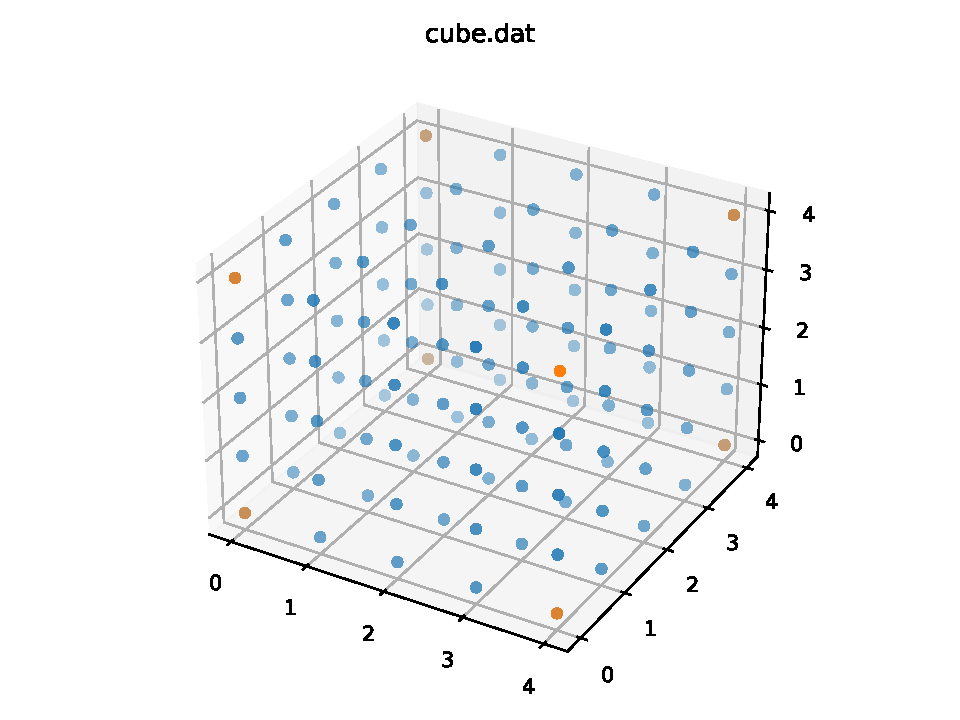
\includegraphics[width=\textwidth]{cube.pdf}
        \caption{Data points from \texttt{cube.dat}, with the eight corners in orange}
        \label{fig:cube}
    \end{subfigure}
    %
    \begin{subfigure}{0.49\linewidth}
        \centering
        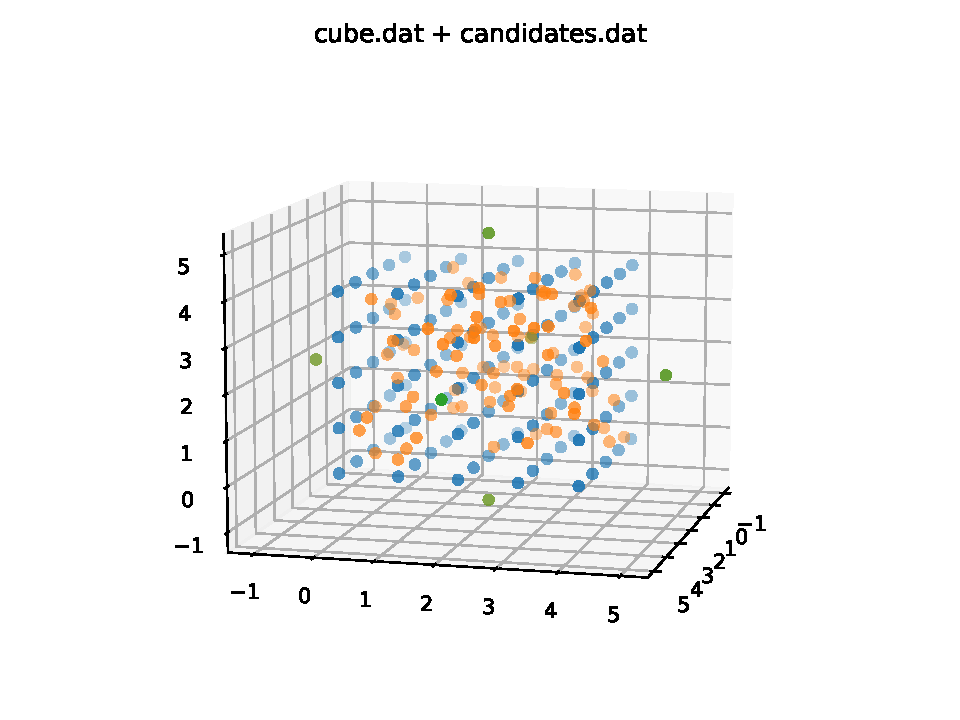
\includegraphics[width=\textwidth]{candidates.pdf}
        \caption{Data points from \texttt{cube.dat} in blue and \texttt{candidates.dat} in orange, with the 6 outer points in green}
        \label{fig:candidates}
    \end{subfigure}
    \caption{}
\end{figure}

There are two example data sets that were mainly used for testing and demo purposes.
The first, \texttt{cube.dat}, is a set of points on a cubic lattice, as shown in Figure \ref{fig:cube}.
For $n = 8$ the subset of points that are maximally separated are, of course, the 8 corners.
Using \texttt{select\_data} to select 8 points will find these corners, assuming a reasonable choice for initial temperature.

The second data set, \texttt{candidates.dat}, is a set of random points that lie ``inside'' the cubic lattice in \texttt{cube.dat}, and six additional points outside the six faces of the cube.
All of these points are shown in Figure \ref{fig:candidates}.
For $l = 6$ adding these six outer points to the cubic lattice results in the maximally separated choice.
Using \texttt{add\_data} to add 6 points from \texttt{candidates.dat} to \texttt{cube.dat} will find these outer points, assuming a reasonable choice for initial temperature.

\end{document}
